\documentclass[12pt, a4paper, twoside, openright]{book}

\usepackage{vuwthesis} % sets up some local things, mostly the front page

\usepackage{palatino} % sets palatino as the default font

\usepackage{url} % for typesetting urls

\usepackage{graphicx}
\usepackage{amsmath}
\usepackage{amssymb}
\usepackage{hyperref}
\DeclareUnicodeCharacter{2212}{-}
\providecommand{\tightlist}{%
  \setlength{\itemsep}{0pt}\setlength{\parskip}{0pt}}

%\renewcommand{\baselinestretch}{1.00}


\begin{document}

\frontmatter
% Book style knows about front matter
% Report style doesn't so you need to set roman numbering etc yourself :-(

%%%%%%%%%%%%%%%%%%%%%%%%%%%%%%%%%%%%%%%%%%%%%%%%%%%%%%%

\title{ABSTRACTION FOR EFFICIENT REINFORCEMENT LEARNING}
\author{Alexander Telfar}

\subject{Computer Science}
\abstract{An abstract of fewer than 500 words must be included.}
% Books don't normally have abstracts, and this is a bit of a hack

% Uncomment the appropriate degree
% \phd
\mscthesisonly
% \mscwithhonours
%\mscbothparts
% \otherdegree{DEGREE OR DIPLOMA NAME}



%%%%%%%%%%%%%%%%%%%%%%%%%%%%%%%%%%%%%%%%%%%%%%%%%%%%%%%




\maketitle

\chapter*{Acknowledgments}\label{C:ack}

Mostly, I would like to thank my advisers: Will Browne, for supporting my work and giving me the freedom to explore my interests.
And Brendan McCane for timely feedback.

I would like also to thank Daniel Braithwaite, Marcus Frean and Stephen Marsland
for their friendship, humour and intellectual support.
And, I would like to thank my family (Ian and Evee), who, for some reason, put up with me.

And finally, I am thankful that SFTI supports theoretical work, despite its high risk.

% also thankful for ...? arms, eyes, health, purpose, money, safety, ... a long list.


\tableofcontents


%%%%%%%%%%%%%%%%%%%%%%%%%%%%%%%%%%%%%%%%%%%%%%%%%%%%%%%

% book style knows about mainmatter
% if you are using report style you will have to rest page numbering etc.
\mainmatter

%%%%%%%%%%%%%%%%%%%%%%%%%%%%%%%%%%%%%%%%%%%%%%%%%%%%%%%

% individual chapters included here

\chapter{Introduction}\label{C:intro}

% RL is inefficient
Reinforcement learning has an efficiency problem: AlphaGo \cite{Silver2016a}, the Go
playing AI that beat world champion Lee Sedol, needed 1.28 million games, with
extra supervision from another 29.4 million positions, using 50 GPUs.
OpenAI Five \cite{OpenAI2018}, the Dota 2 playing AI that beat OG, the winners of TI8/9, was
trained over 10 months, at it peak, collecting 900 years of experience per day, using
128,000 CPUs and 256 GPUs. Is RL fundamentally expensive, or can we do better?

% Existing theory tells us ...
Bounds on sample and computational complexity tell us that !??!

% What strategies are there to improve the efficiency of RL?

\chapter{MDPs}

What is a decision problem?
Why do we care?

\hypertarget{sequential-decision-problems}{%
\section{Sequential decision
problems}\label{sequential-decision-problems}}

% MDPs are a subset of sequential decision problem. Define MDPs. Give
% example.

A MDP is defined as a tuple, \(\{\mathcal S, \mathcal A, P(s_{t+1} \mid s_t, a_t),R(s_t, a_t, s_{t+1}), \gamma\}\)\footnotemark[1]. Where \(s \in \mathcal S\) is the set of possible states (\textit{for example arrangements of chess pieces}), \(a \in \mathcal A\) is the set of actions (\textit{the different possible moves, left, right, diagonal, weird L-shaped thing, ...}),  \(P(s_{t+1} \mid s_t, a_t)\) is the transition function which describes how the environment acts in response to the past (\(s_t\)) and to your actions (\(a_t\)) (\textit{in this case, your opponent's moves, taking one of your pieces, and the results of your actions}), and finally, \(r(s_t, a_t, s_{t+1})\) is the reward function, \textit{whether you won (+1) or lost (-1) the game }.
The objective when solving a MDP is to find a policy, $\pi(a_t | s_t)$, that maximises the discounted cumulative reward, \(R =\sum_{t=0}^T \gamma^t r(s_t, a_t, s_{t+1}) \).

\footnotetext[1]{Why is the discount factor a part of the definition of the MDP?
By defining the discount it ensures the MDP has a unique solution.}

If we wanted we could pick our actions before we make observations,
reducing the search space to only \(|A| \times T\). But this is a bad idea\ldots{} example.

The general feeling of an MDP. - Actions need to be adapted to new
observations and contexts. - While instantaneous results are good, we
care about the longer term aggregates.

\hypertarget{the-markov-property}{%
\subsection{The Markov property}\label{the-markov-property}}

\begin{displayquote}
  What does the M in MDP really mean?
\end{displayquote}

When we say a decision problem is Markovian, we mean that the transition
function generates a Markov chain. The next transition step depends only
on the current state and action. It is invariant to any and all histories that do not
change the current state.

This is not to say that past actions do not effect the future. Rather,
it is a special type of dependence on the past. Where the dependence is
totally described by changes to the \textbf{observable} state.

% Can easily make a sequence Markovian by adding information. E.g.
% time

When actions you have taken in the past can bite you in the butt \ldots{}
Maze with pendulums / doors. When moving through the maze, you must
swing the pendulums. In the future you must avoid being hit. (maybe make
a picture of this?) also, is there a more general way to think about it?

\hypertarget{optimality}{%
\subsection{Optimality}\label{optimality}}

\begin{displayquote}
  \textit{What does it mean to solve an MDP?}
\end{displayquote}

And importantly, existing theory tells us that there is a unique optima to the bellman iterations.
And that this optimal policy(ies) is(are) necessarily deterministic.

(why does this make sense?)


How do we know one policy is better than another? How do we know a
policy is optimal?

\[
\forall \pi\;\; V^{\pi^* } \ge V^{\pi} \\
\]

But, this definition of optimality implicitly assumes a uniform
distribution over states. This is unlikely. Rather, the distribution is
determined by the policy.

\[
\mathop{{\mathbb E}}_{s\sim D_{\pi}} \big[ V^{\pi^* } \big] \ge \mathop{{\mathbb E}}_{s\sim D_{\pi}} \big[ V^{\pi} \big] \\
D_{\pi}(s) = P(s | \pi) = \sum_{\text{all } \tau \text{ with } s_t = s} P(\tau | \pi)
\]

Now. How different is this?

I can imagine some degenerate solutions now being possible? Because we
can control the distribution we are being evaluated on. We could pick a
policy that oscillates between two states, never leaving the cycle.
Therefore it would have \(p(s_1) = p(s_2) = 0.5\) and
\(p(s_{i \neq 1,2}) = 0\).

That doesn't seem so bad?

\begin{displayquote}
  \textit{How hard is it to solve an MDP?}
\end{displayquote}

% Insert lower bound and some intution

\begin{align*}
Q^{\pi}(s_0, a_0) = r(s_0, a_0) &+ \gamma \mathop{\text{max}}_{a_1} \mathop{\mathbb E}_{s_1\sim p(\cdot | s_0, a_0)} \Bigg[ \\
r(s_1, a_1)  &+ \gamma \mathop{\text{max}}_{a_2} \mathop{\mathbb E}_{s_2\sim p(\cdot | s_1, a_1)} \bigg[\\
r(s_2, a_2)  &+ \gamma \mathop{\text{max}}_{a_3} \mathop{\mathbb E}_{s_3\sim p(\cdot | s_2, a_2)} \Big[
\dots \Big] \bigg] \Bigg]
\end{align*}

\hypertarget{how-do-mdps-relate-to-rl}{%
\section{How do MDPs relate to RL?}\label{how-do-mdps-relate-to-rl}}

Reinforcement learning refers to the set of solutions to a type of problem.
This general, reinforcement learning, problem, has two main properties;
\textit{"trial-and-error search and delayed rewards"} \cite{Sutton2018}.
Unlike supervised learning, which gives the learner feedback (\textit{Student: "I think that digit
is a 5". Teacher: "No, it's a 6"}), in RL the learner only receives evaluations (\textit{Student: "I think
that digit is a 5". Teacher: "No."}). This means the student needs to explore the possible answers via some trial-and-error search.
(\textit{Student: "Is it a 4?". Teacher: "No." Student: "How about a 0?". Teacher: "No." ... Student: "A 6?". Teacher: "Yes."})

Ontop of terse teachers, many actions may be taken
before any evaluation is received, thus requiring credit to be assigned to actions,
often leaving the learner wondering: "what did I do to deserve this?" (see
\href{https://www.youtube.com/watch?v=Qv4H81gEGDQ}{pigeon superstition} for an amusing
example of credit assignment gone wrong \cite{Box1997}).

% Your teaher might only give you evaluations for sequences of actions, rather than individual actions.
% Thus you are left with trying to infer how these sequence evaluations tells you about which actions you should take.

The above definition of reinforcement learning is quite general. There are many
different dimensions to problems that have the properties trial-and-error search and
delayed feedback. For example we could make a RL problem that is;

\begin{itemize}
\tightlist
\item
  Observable or un-observable
\item
  Deterministic or stochastic
\item
  Synchronous or asynchronous
\item
  Terminating or infinite
\item
  Discrete versus continuous
\item
  Given knowledge of the underlying model
\end{itemize}


% MDPs are also within the fields of Operational Research, Optimal Control, Mathematical
% Optimisation, Stochastic Programming.


\section{The simplest RL setting}

\begin{displayquote}
  \textit{What is the minimally complex setting we can consider that still poses an
  interesting challenge to the ML / RL communities?}
\end{displayquote}

\hypertarget{a-tabular-representation-of-mdps}{%
\subsection{A tabular representation of MDPs}\label{a-tabular-representation-of-mdps}}

Imagine a tabular MDP, where we can describe the MDP with tables.
A table of three dimensions can describe the transition probabilities, $P[s_{t+1}, s_t, a_t]$,
and a table of two dimensions can describe the rewards, $r[s_t, a_t]$: the states and actions
act as indexes to locations in the tables.

Consider a tabular MDP with deterministic actions, where $P(s_{t+1}|s_t, a_t) \in \{ 0, 1\}$.
This RL problem can be efficiently solved by non-statistical
methods: dynamic programming and related planning techniques \cite{Bertsekas1995}.

But, a tabular MDP with stochastic actions, $P(s_{t+1}|s_t, a_t) \in [0, 1]$,
seems to retain much of the complexity we care about. This setting does not allow
efficient solutions via dynamic programming. And can be approached with algorithms
that are used for state-of-the-art DRL such as policy gradients,

Let's more formally define our tabular MDP.

\begin{align}
\mathcal M &= \{S, A, P, r, \gamma\} \\
S &= [0:n-1] \\
A &= [0:m-1] \\
P &\in [0,1]^{n\times n \times m}, \;\;\forall j, k : \sum_i P[i, j, k] = 1 \\
r &\in \mathbb R^{n\times m}
\end{align}

A result of this formulation is that we consisely write and solve the Bellman equation analytically.

\begin{align}
V &= r_{\pi} + \gamma P_{\pi} V \tag{the bellman eqn}\\
V - \gamma P_{\pi} V &= r_{\pi}\\
(I-\gamma P_{\pi})V &= r_{\pi}\\
V &= (I-\gamma P_{\pi})^{-1}r_{\pi}
\end{align}

The values are written as a vector, $V \in \mathbb R^n$.
The reward under a given policy is written $r_{\pi}[s, a] = \pi[s, a] r[s, a]$.
And the transitions under a given policy is written $P_{\pi}[s', s] = \sum_a P[s', s, a]\pi[s, a]$.


\subsection{The value function polytope}

The value function polytope \cite{Dadashi2018} is the


Imagine a two state MDP. Following some initial, ill-informed policy,
the value that you might get starting from either state state is $v_1, v_2$.



\begin{figure}
\centering

\includegraphics[width=1\textwidth,height=0.25\textheight]{../../pictures/drawings/2-state-automata.png}
\caption{Consider the simplest possible MDP, with two states and two actions. (Any simpler setting is entierly uninteresting. A single state means actions do nothing.
And a single action means all policies are the same...).}
\end{figure}


% \begin{figure}
% \centering
% 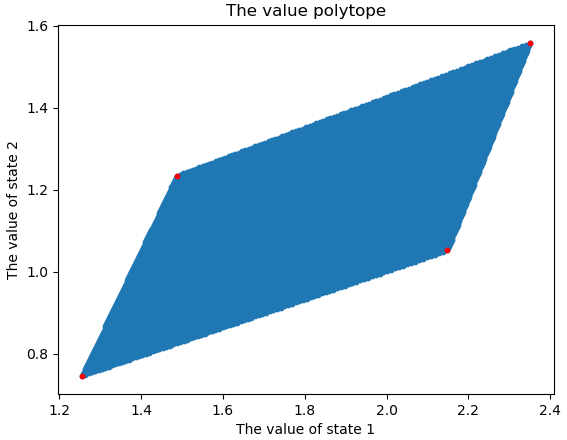
\includegraphics[width=1\textwidth,height=0.25\textheight]{../../pictures/drawings/value-polytope.png}
% \caption{The value polytope for a two state, two action MDP.}
% \end{figure}

\chapter{Abstraction}\label{C:bin}


\hypertarget{solveable-representations}{%
\section{Solveable representations}\label{solveable-representations}}

\begin{quote}
Representations with structure that is easily solvable.
\end{quote}

While there are other ways to add exploitable structure, here we only
consider linearity.

The bellman equation is a non-linear optimisation problem. It does have
some nice properties, like having a unique optima under the bellman
operator. But, in general, it isn't very friendly. Is there a way to
turn this into a linear problem? What sacrifices need to be made to
achieve this?

\hypertarget{why-linearity}{%
\subsubsection{Why linearity?}\label{why-linearity}}

\begin{itemize}
\tightlist
\item
  it has many mathematical tools for analysis.
\item
  we know linear systems can be solved efficiently.
\item
  ?
\end{itemize}

Linearity is a nice property that makes optimisation simpler and more
efficient.

\begin{itemize}
\tightlist
\item
  Linear programming (see appendix: LP)
\item
  Linear markov decision processes
\end{itemize}

Solving a system of linear relationships. Has a complexity of ???.

In fact. MDPs can actually be solved via LP. see {[}appendix{]}.

\hypertarget{a-closer-look-at-lmdps}{%
\subsubsection{A closer look at LMDPs}\label{a-closer-look-at-lmdps}}

(the Todorov ones\ldots{})

The three steps of abstraction - relaxation (transform to a new domain)
- linearisation (and solve) -

\hypertarget{lmdps-more-formally}{%
\paragraph{LMDPs; more formally}\label{lmdps-more-formally}}

\begin{figure}
\centering
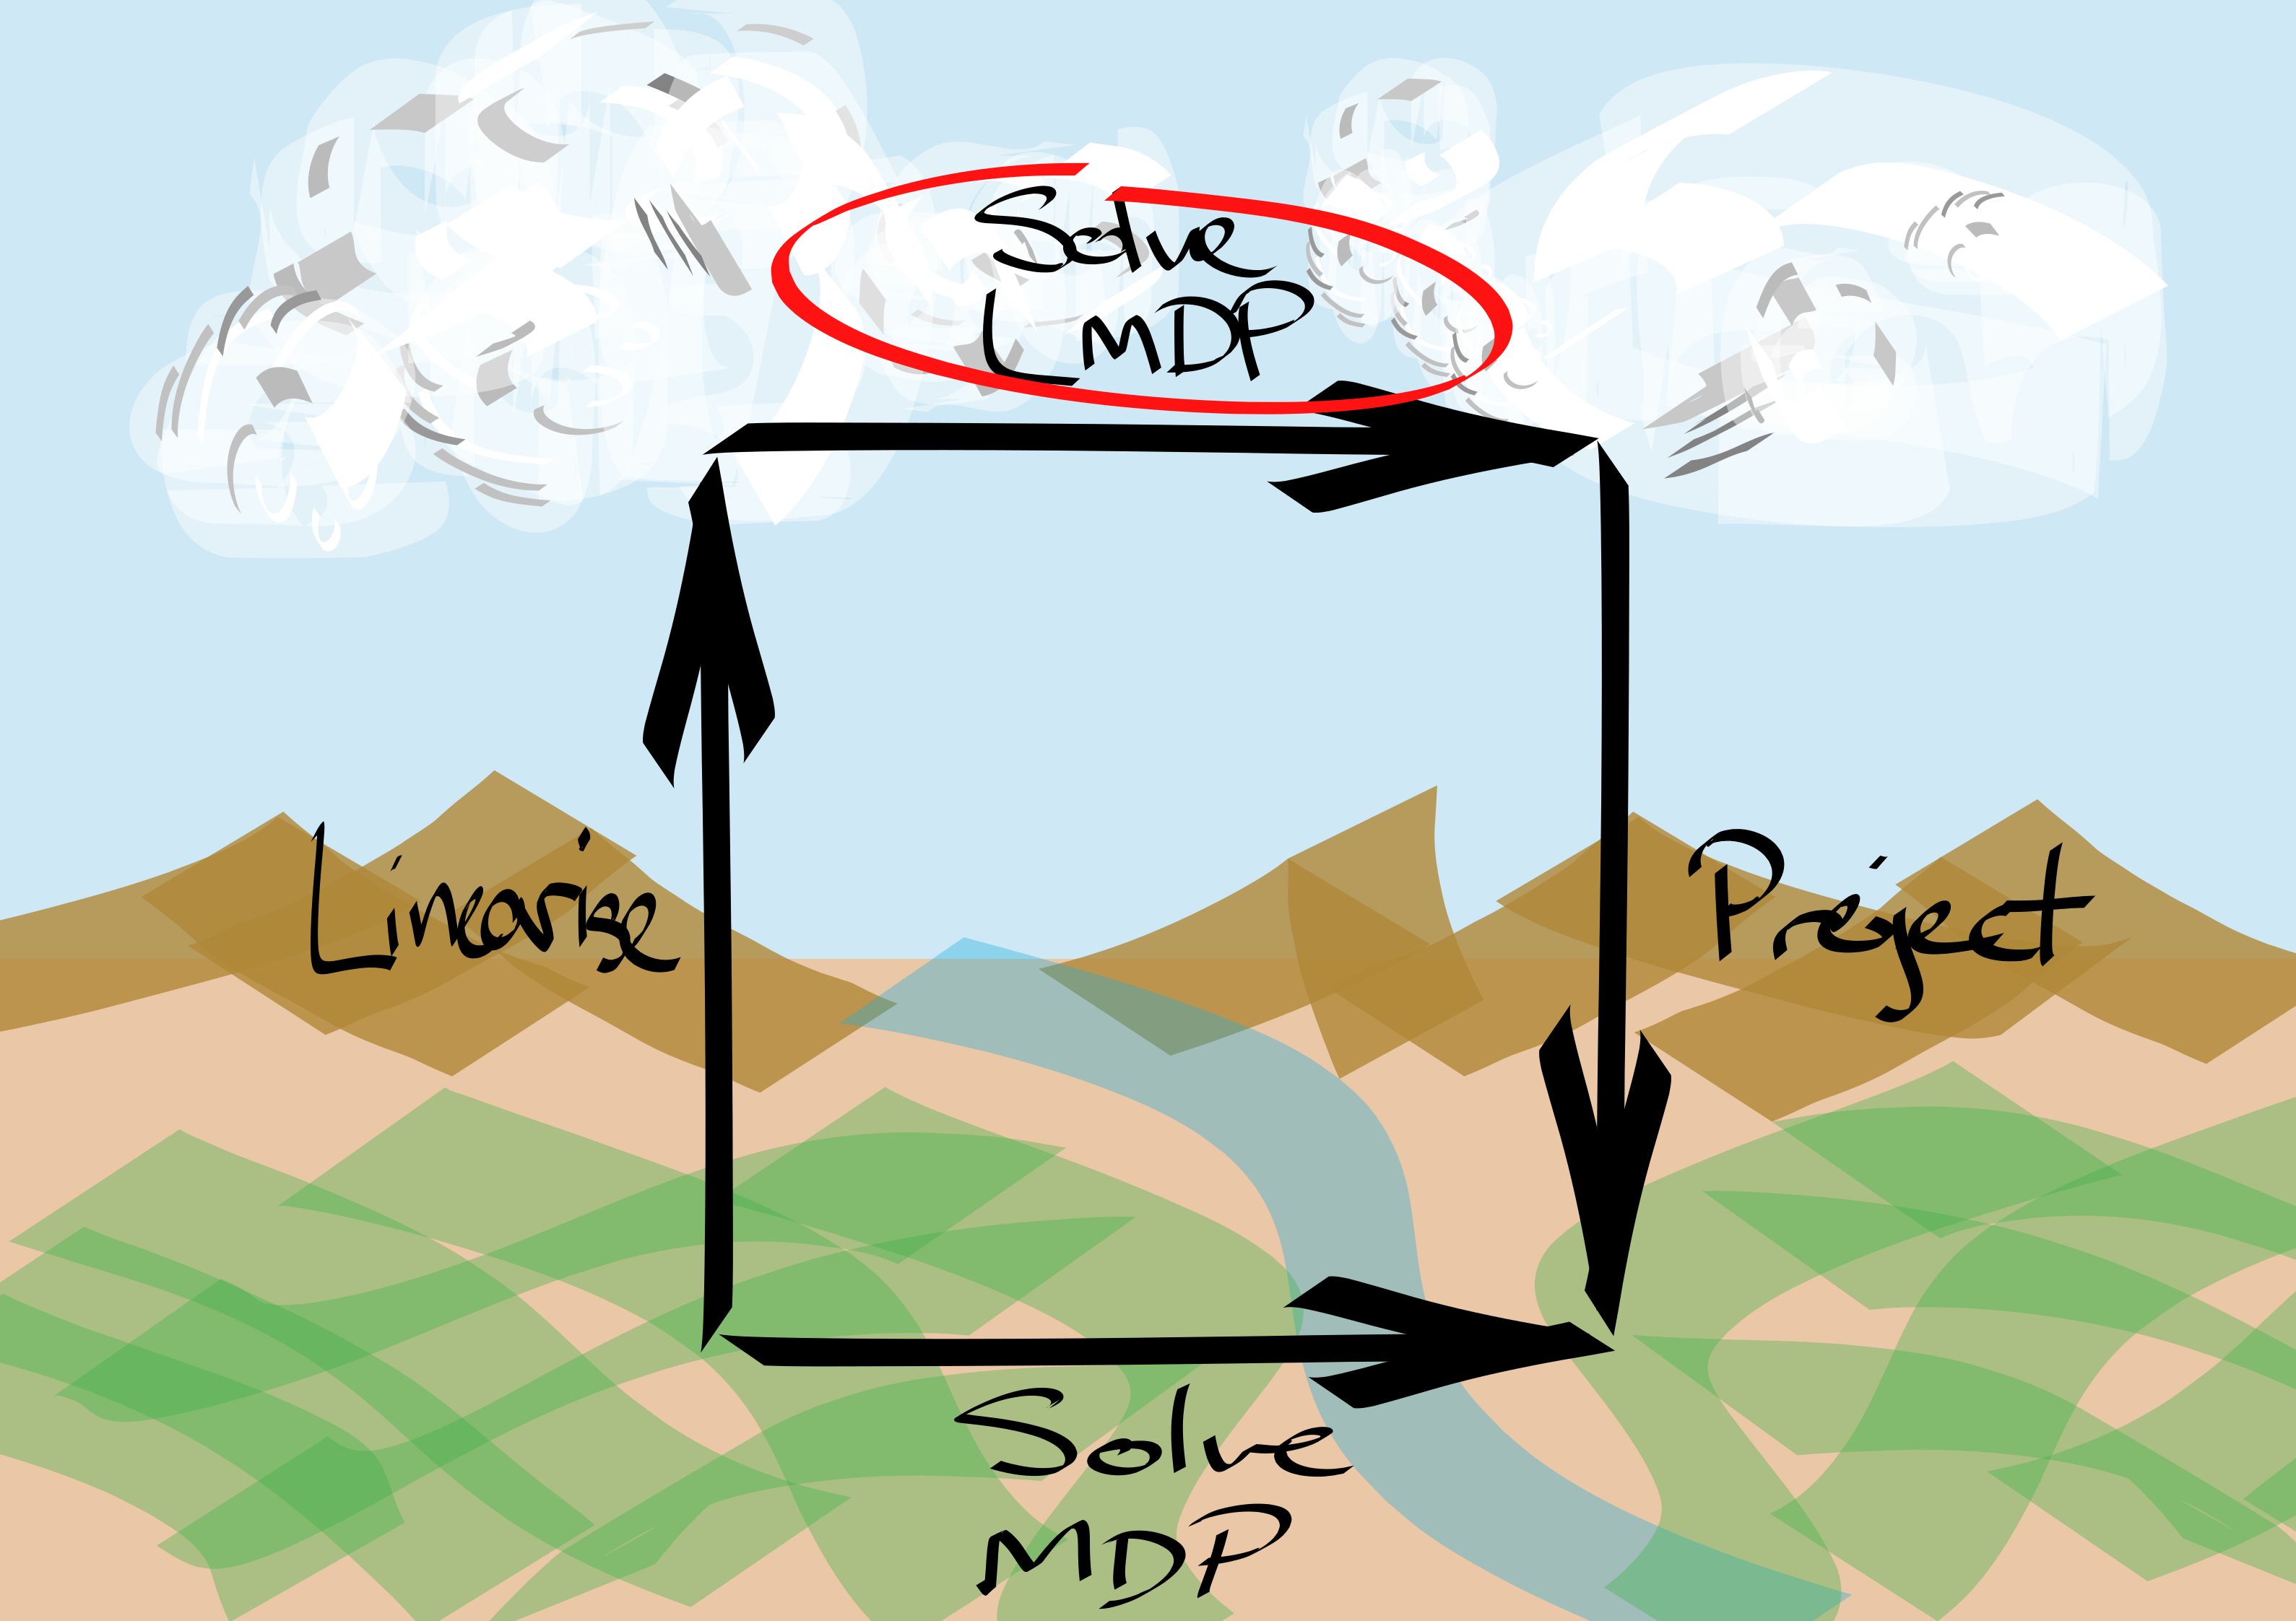
\includegraphics[width=0.5\textwidth,height=0.5\textheight]{../../pictures/drawings/abstract-representations-solve.png}
\caption{''}
\end{figure}

Pick \(a \in A\), versus, pick \(\Delta(S)\). \(f: S\to A\) vs
\(f:S \to \Delta(S)\).

In the original Todorov paper, they derive the LMDP equations for
minimising a cost function. This maximisation derivation just changes a
few negative signs around. Although there is also a change in the
interpretation of what the unconstrained dynamics are doing. \ldots{}?

\begin{align}
V(s) &= \mathop{\text{max}}_{u} q(s) - \text{KL}(u(\cdot| s) \parallel p(\cdot | s)) + \gamma \mathop{\mathbb E}_{s' \sim u(\cdot | s)} V(s') \tag{1}\\
\\
u^{* }(\cdot | s) &= \frac{p(\cdot | s)\cdot z(\cdot)^{\gamma}}{\sum_{s'} p(s' | s) z(s')^{\gamma}} \tag{8}\\
z_{u^{* }} &= e^{q(s)}\cdot P z_{u^{* }}^{\gamma} \tag{11}\\
\end{align}

By definition, an LMDP is the optimisation problem in (1). (3) Define a
new variable, \(z(s) = e^{v(s)}\). (5) Define a new variable that will
be used to normalise \(p(s' | s)z(s')^{\gamma}\). (8) Set the optimal
policy to minimise the KL distance term. (9) Since we picked the optimal
control to be the form in (8), the KL divergence term is zero. (11)
Rewrite the equations for the tabular setting, giving a \(z\) vector,
uncontrolled dynamics matrix.

(see appendix {[}{]} for a full derivation)

\hypertarget{a-relaxed-mdp}{%
\paragraph{A relaxed MDP}\label{a-relaxed-mdp}}

\begin{figure}
\centering
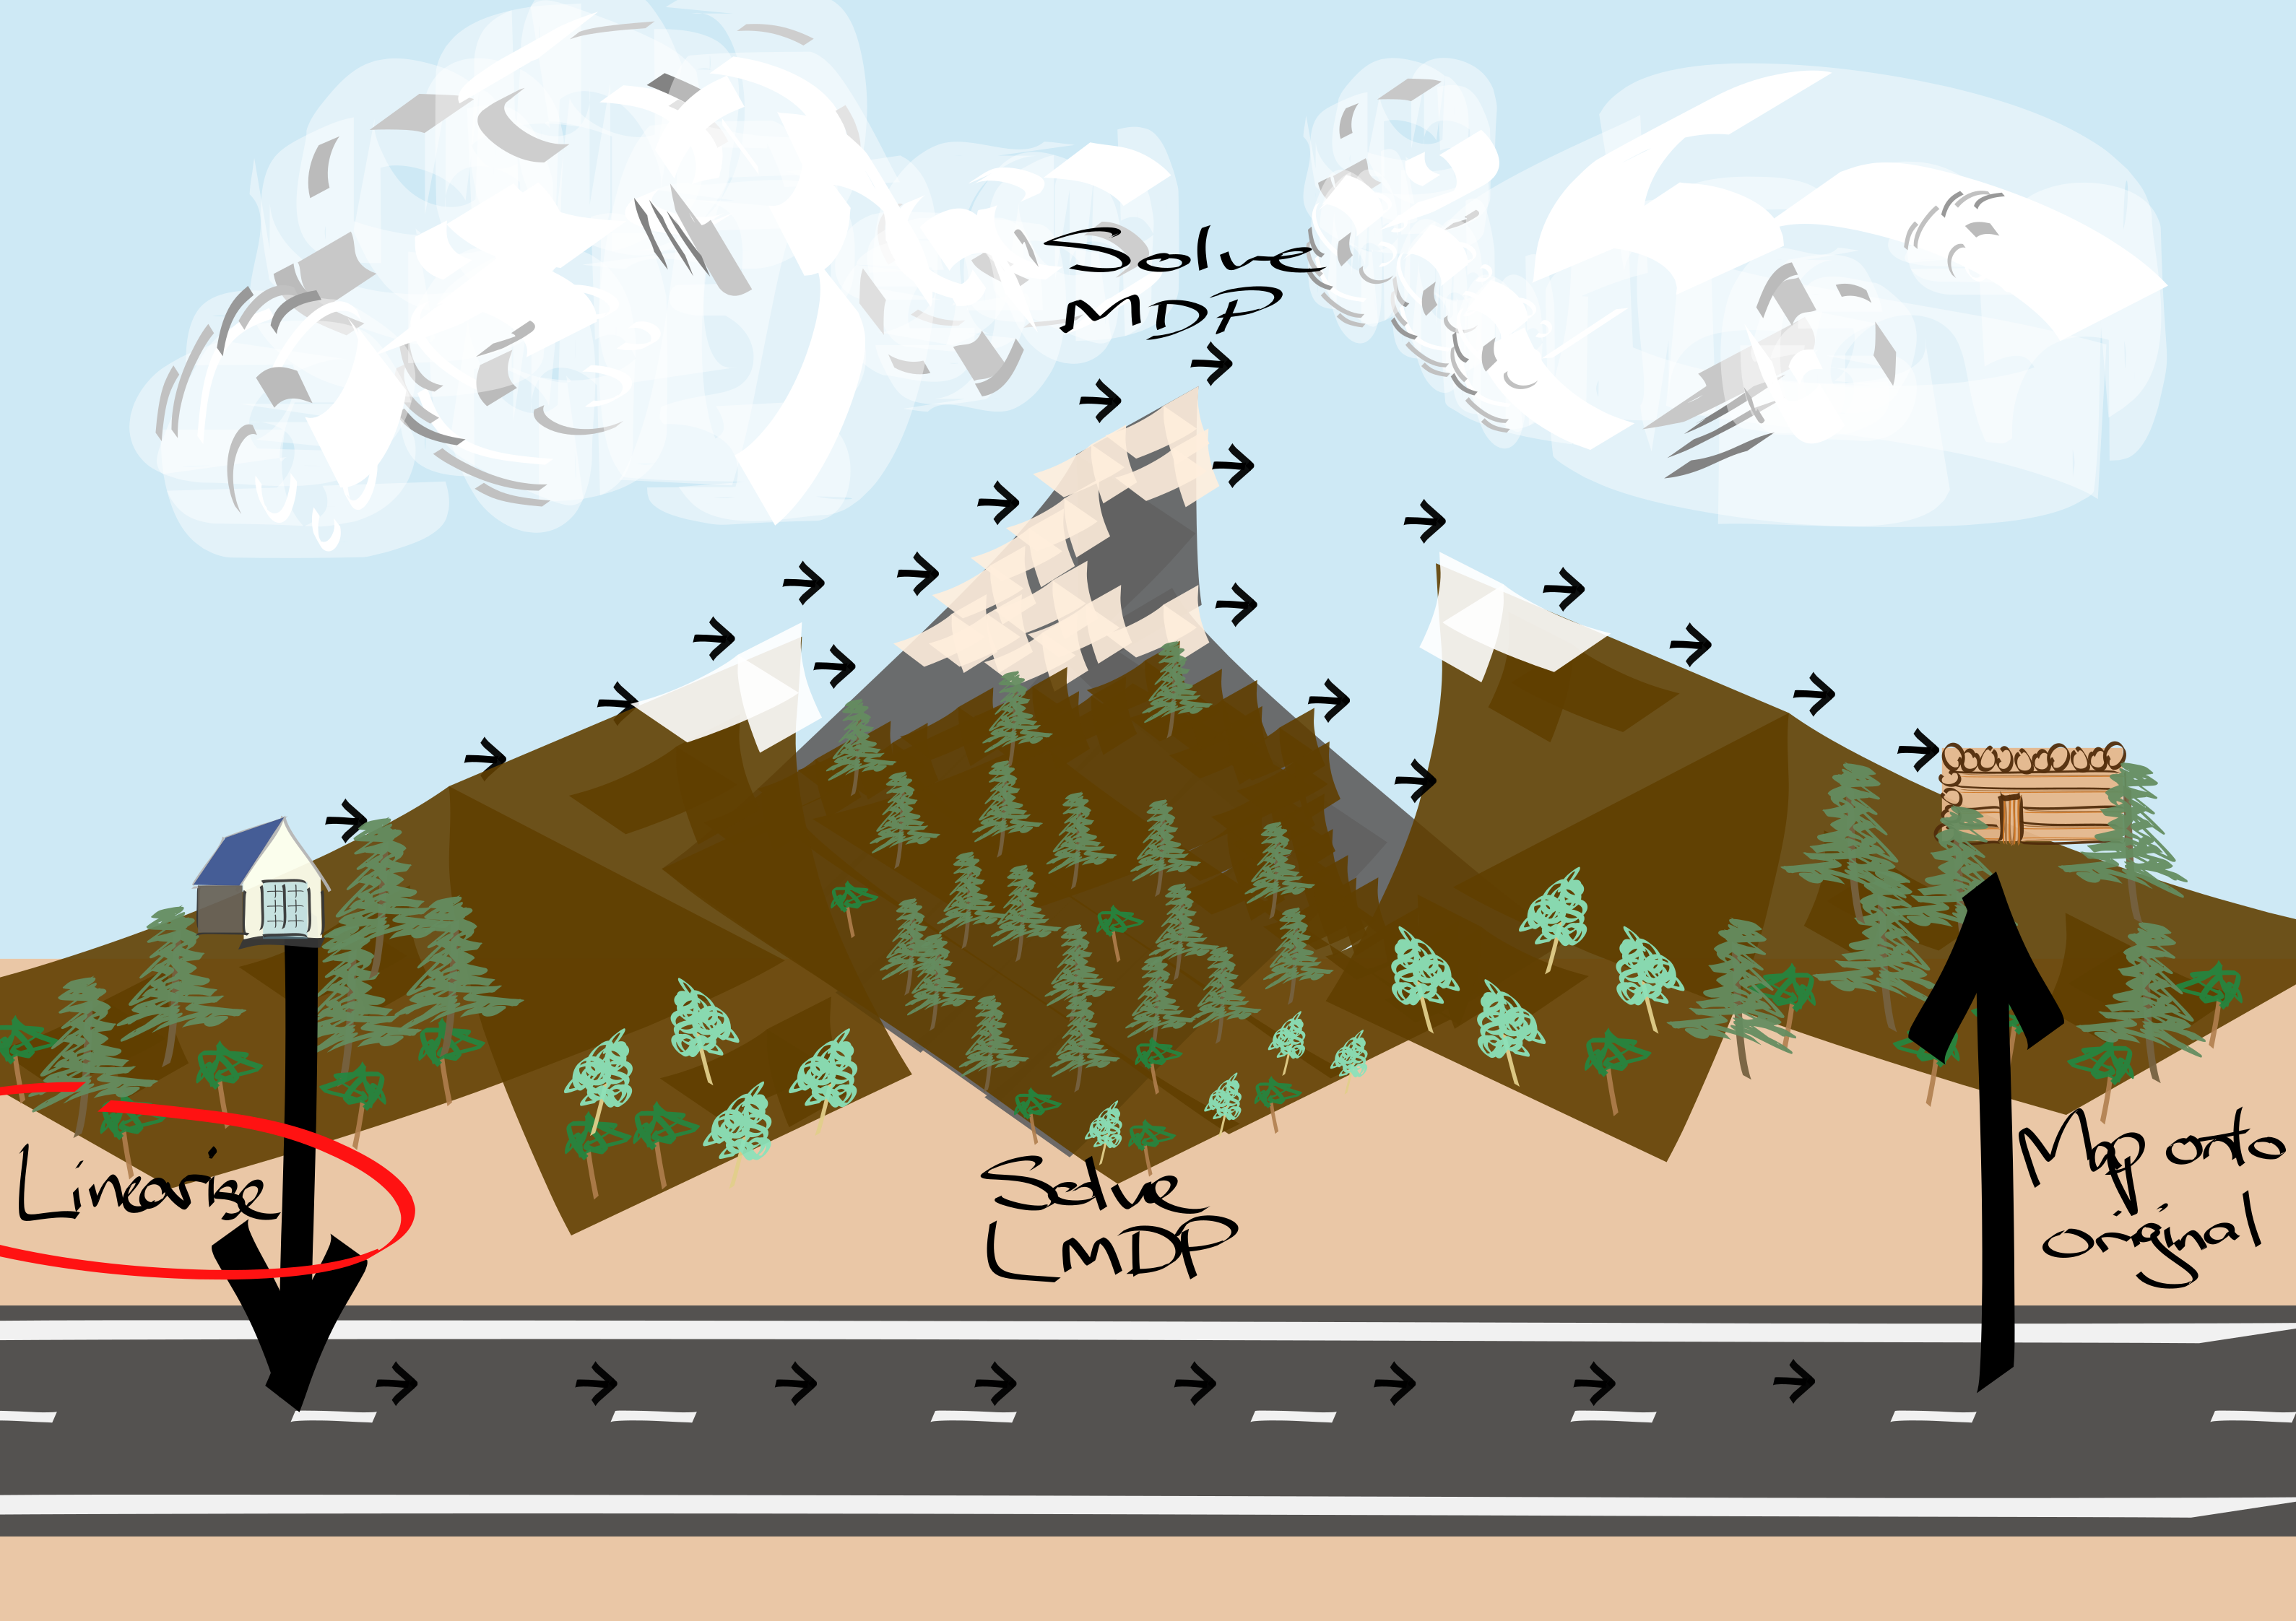
\includegraphics[width=0.5\textwidth,height=0.5\textheight]{../../pictures/drawings/abstract-representations-linear.png}
\caption{''}
\end{figure}

\begin{quote}
Ok great, we can solve LMDPs. But how does being able to solve an LMDP
help us solve MDPs?
\end{quote}

We want a way to transform a MDP into a LMDP, while preserving the
`structure' of the MDP. But what do we mean by a MDP's structure?

The LMDP, \(\{S, p, q, \gamma\}\) should;

\begin{itemize}
\tightlist
\item
  be able to represent the same transition dynamics as the original MDP,
\item
  give the the same rewards was the original MDP,
\item
  have the same optima.
\end{itemize}

(It turns out that (1) and (2) imply (3) given some assumptions. See
\href{}{Optimality})

So, given a reward function, \(r\), and a transition function, \(P\),
from the MDP, we must translate them into a \(p\) and a \(q\). Thus we
have built a LMDP with the same `structure'.

\begin{align}
\forall s, s' \in S, \forall a \in A, \exists u_a& \;\;\text{such that;} \\
P(s' | s, a) &= u_a(s'|s)p(s'|s) \tag{1}\\
r(s, a) &= q(s) - \text{KL}(P(\cdot | s, a) \parallel u_a(\cdot| s) ) \tag{2}\\
\end{align}

Which leads to \(|A|\) linear equations to solve, for each state in the
MDP.

See appendix {[}{]} for more details.

Alternative views of linearisation.

\begin{itemize}
\tightlist
\item
  A relaxation of the MDP
\item
  Linelihood interpretation
\end{itemize}

\hypertarget{unconstrained-dynamics-and-state-rewards}{%
\subparagraph{Unconstrained dynamics and state
rewards}\label{unconstrained-dynamics-and-state-rewards}}

\begin{quote}
Let's try and understand this thing we have contructed.
\end{quote}

The state rewards are not capable of giving rewards for actions taken.
Rather, the differences in reward, by taking another action, is captured
by the KL divergence between the control and the unconstrained dynamics.

\begin{itemize}
\tightlist
\item
  What is their function?
\item
  What do they look like?
\end{itemize}

Does it make sense to treat the q(s) like rewards?! They reward for bing
in state s. But cant capture action specific rewards!?

\hypertarget{decoding}{%
\paragraph{Decoding}\label{decoding}}

\begin{figure}
\centering
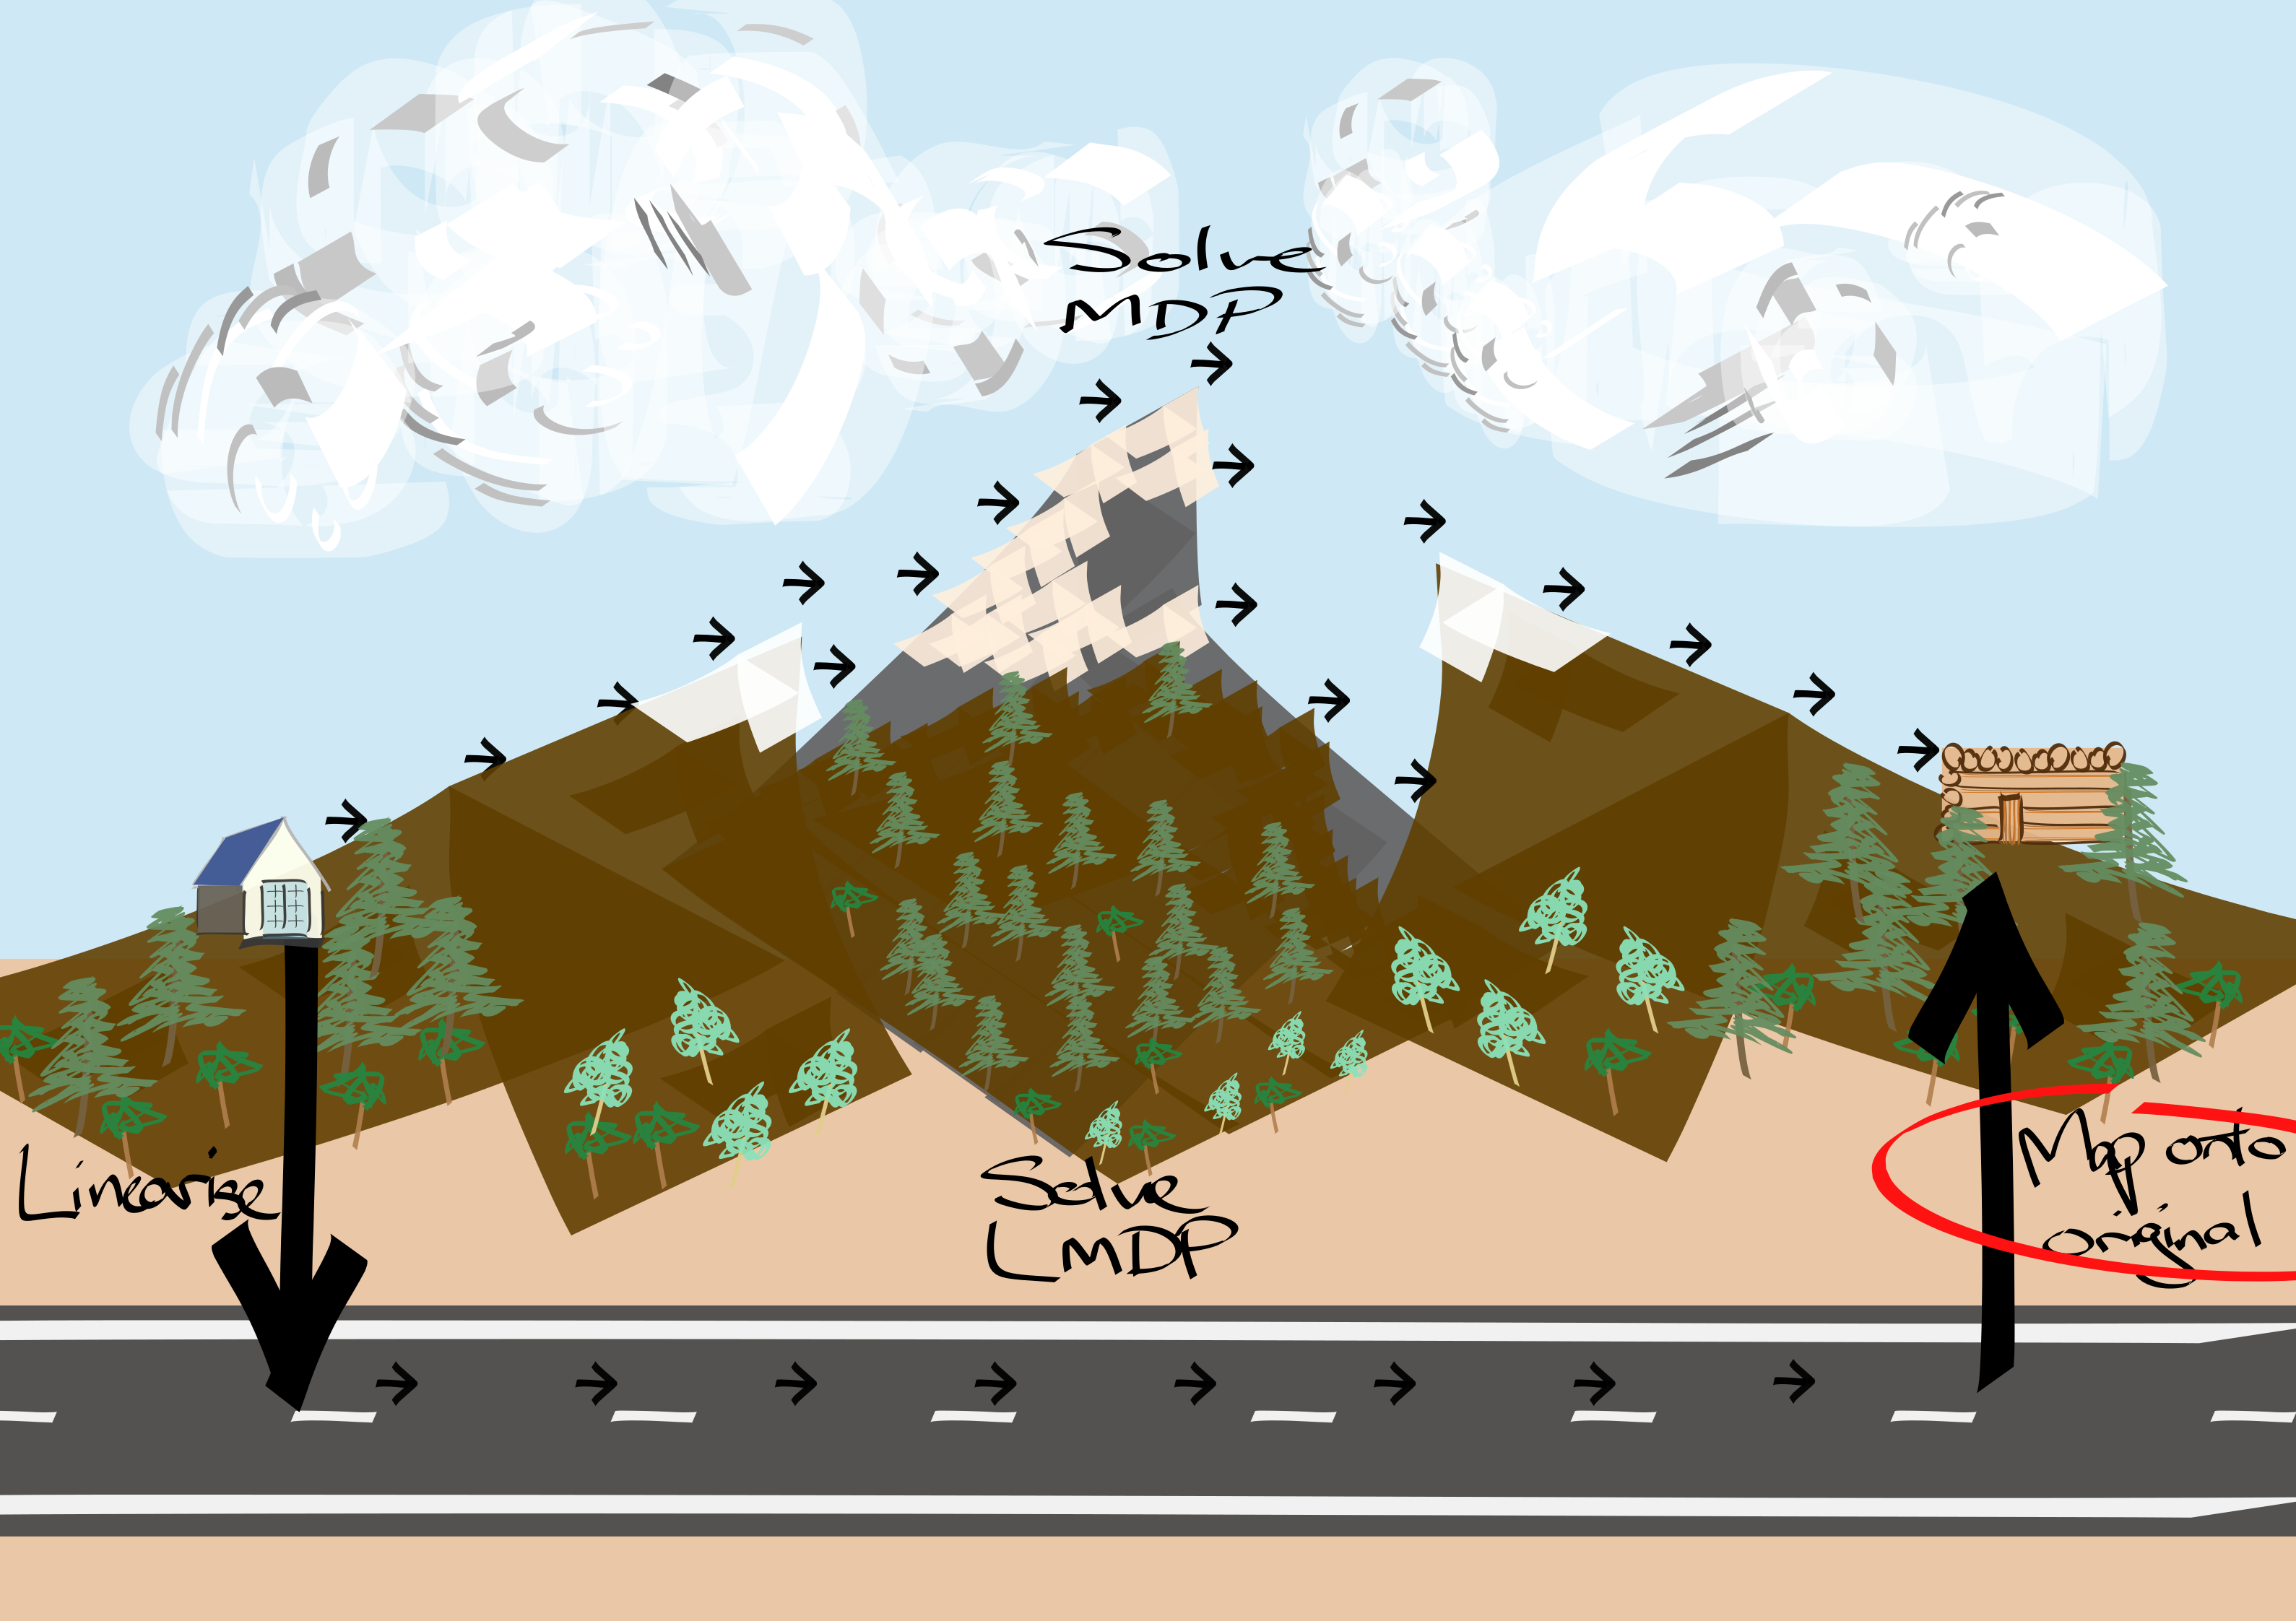
\includegraphics[width=0.5\textwidth,height=0.5\textheight]{../../pictures/drawings/abstract-representations-project.png}
\caption{''}
\end{figure}

Ok, so now we get a glimpse at why LMDPs are an interesting abstraction.
THe LMDP has disentangled the search for the behaviour (go to this or
that state) and the search for optimal controls (how to actually achieve
that behaviour). This can be seen in the decoding step. As we know which
states we want to be in, via the optimal control from solving the LMDP,
\(u^{* }\), but, we do not know how to implement those controls using
the actions we have available.

\begin{quote}
Two `simpler' problems. Easier to solve?
\end{quote}

\begin{align}
P_{\pi}(\cdot | s) = \sum_a P(\cdot | s, a) \pi(a | s) \\
\pi = \mathop{\text{argmin}}_{\pi} \text{KL}\Big(u(\cdot | s))\parallel P_{\pi}(\cdot | s)\Big)
\end{align}

Maybe this isnt enough? Do we need to add a reward sensitive part as
well?!? (but what if the actual path we take to get there has a neg
rewards?!?)

\hypertarget{optimality-of-solutions-via-lmdps}{%
\paragraph{Optimality of solutions via
LMDPs}\label{optimality-of-solutions-via-lmdps}}

\begin{quote}
Do these two paths lead to the same place?
\end{quote}

One of the main questions we have not addressed yet is; if we solve the
MDP directly, or linearise, solve and project, do we end up in the same
place? This is a question about the completeness of our abstraction. Can
our abstraction represent (and find) the same solutions that the
original can?

\begin{align}
\parallel V_{\pi^{* }} - \parallel V_{\pi^{* }} - V_{\pi_{u^{* }}} \parallel_{\infty}&= \epsilon  \tag{1}\\
&=\parallel (I - \gamma P_{\pi^{* }})^{-1}r_{\pi^{* }} - (I - \gamma P_{\pi_{u^{* }}})^{-1}r_{\pi_{u^{* } }} \parallel_{\infty} \tag{2}\\
&\le\parallel (I - \gamma P_{\pi^{* }})^{-1}r - (I - \gamma P_{\pi_{u^{* }}})^{-1}r \parallel_{\infty} \tag{3}\\
&=\parallel \bigg((I - \gamma P_{\pi^{* }})^{-1} - (I - \gamma P_{\pi_{u^{* }}})^{-1} \bigg) r \parallel_{\infty} \tag{4}\\
&\le r_{\text{max}} \parallel (I - \gamma P_{\pi^{* }})^{-1} - (I - \gamma P_{\pi_{u^{* }}})^{-1}   \parallel_{\infty} \tag{5}\\
&= r_{\text{max}} \parallel \sum_{t=0}^{\infty} \gamma^t P_{\pi^{* }} - \sum_{t=0}^{\infty} \gamma^t P_{\pi_{u^{* }}}  \parallel_{\infty} \tag{6}\\
&= r_{\text{max}} \parallel \sum_{t=0}^{\infty} \gamma^t (P_{\pi^{* }} - P_{\pi_{u^{* }}})   \parallel_{\infty} \tag{7}\\
&= \frac{r_{\text{max}}}{1-\gamma} \parallel P_{\pi^{* }} - P_{\pi_{u^{* }}} \parallel_{\infty} \tag{7}\\
\end{align}

\begin{enumerate}
\def\labelenumi{(\arabic{enumi})}
\tightlist
\item
  We want to compare the optimal policies value and the value achieved
  by the optimal LDMP solution.
\item
  Assume that there exists a policy that can generate the optimal
  control dynamics (as given by the LMDP). In that case we can set
  \(P_{\pi_{u^{* }}} = U^{* }\).
\item
  \(r_{u^{* }}\) doesnt really make sense as the reward is action
  dependent. We could calculate it as \(r_{\pi_{u^{* } }}\), but we dont
  explicity know \(\pi_{u^{* }}\). \((I - \gamma P_{\pi^{* }})^{-1}r\)
  represents the action-values, or \(Q\) values. By doing this exhange,
  we might over estimate the diffference under the infinity norm as two
  non-optimal actions may have larger difference. Also, use the element
  wise infinity norm.
\end{enumerate}

\begin{center}\rule{0.5\linewidth}{\linethickness}\end{center}

Ok, great. Insights from optimality bounds.

Need to be able to approximate the optimal controls. When is it hard to
approximate the optimal controls? When our basis set of distributions
oer future states (aka our actions) have little weight\ldots{}?

Potential solution? Use options.

\hypertarget{option-decoding}{%
\paragraph{Option decoding}\label{option-decoding}}

What about using options to help solve the optimal control decoding?
Does this actually help?!

\begin{align}
P_{\pi}(\cdot | s) = \sum_\omega P_k(\cdot | s, \omega) \pi(\omega | s) \\
\pi = \mathop{\text{argmin}}_{\pi} \text{KL}\Big(u(\cdot | s))\parallel P_{\pi}(\cdot | s)\Big)
\end{align}

Options would allow greater flexibility in the \(P_{\pi}(\cdot | s)\)
distribution, making is possible to match \(u(s'|s)\) with greater
accuracy (and possibly cost).

\begin{itemize}
\tightlist
\item
  First need to demonstrate that action decoding is lossy.
\item
  Then show that using options is less lossy.
\end{itemize}

This introduces dangers?!? As an option might accumulate unknown rewards
along the way!??

\hypertarget{the-complexity-of-solutions-via-lmdps}{%
\subsubsection{The complexity of solutions via
LMDPs}\label{the-complexity-of-solutions-via-lmdps}}

\begin{quote}
Is my path actually shorter?
\end{quote}

The whole point of this abstraction was to make the problem easier to
solve. So hasit actually made it any easier?

The complexity of solving our abstraction can be broken down into the
three steps;

\begin{itemize}
\tightlist
\item
  linearisation: \(|S| \times \text{min}(|S|,|A|)^{2.3}\)
\item
  solve the LMDP: \(\text{min}(|S|,|A|)^{2.3}\)
\item
  project back: \(???\)
\end{itemize}

Giving a total complexity of \ldots{}

Contrasted with the complexity of solving an MDP.

\hypertarget{scaling-to-more-complex-problems}{%
\subsubsection{Scaling to more complex
problems}\label{scaling-to-more-complex-problems}}

Now that we have some evidence that this LMDP solution strategy makes
sense, it efficiently (see \href{}{complexity}) yields high value (see
\href{}{optimality}) policies. We want to test it out on some real world
problems. But the real world isn't as nice as the setting we have been
working in. There are a few added complexities;

\begin{itemize}
\tightlist
\item
  sample based / incremental
\item
  large / cts state spaces
\item
  sparse rewards
\end{itemize}

So now that we have explored LMDPs, how can we extract their nice
properties into an architecture that might scale to more complex
problems: larger state spaces and action spaces, sparse rewards,
\ldots{}?

\hypertarget{incremental-implementation}{%
\paragraph{Incremental
implementation}\label{incremental-implementation}}

Generalise to a more complex problem. We are only given samples. A first
step to tackling more complex problems.

\hypertarget{model-based}{%
\subparagraph{Model based}\label{model-based}}

Learn \(p, q\) based on samples.

\begin{align}
\mathcal L(\theta, \phi) = \mathop{\mathbb E}_{s, a,} \bigg[ r(s, a) - q_\theta(s) + \text{KL}(p_\phi(\cdot | s) \parallel P(\cdot | s, a)) \bigg]\\
\mathcal L(\theta, \phi) = \mathop{\mathbb E}_{s, r, s'} \bigg[r - q_\theta(s) - p_\phi(s' | s) \log \frac{1}{ p_\phi(s' | s)} \bigg] \\
\end{align}

\begin{center}\rule{0.5\linewidth}{\linethickness}\end{center}

Ok. Lets take a different approach. \textbf{Q:} Why is it a bad idea to
try to do incremental RL with this linearisation trick? Not sure.

\begin{center}\rule{0.5\linewidth}{\linethickness}\end{center}

Alternative perspective. The high value trajectories are the most likely
ones.

\hypertarget{distributions-over-states}{%
\subsubsection{Distributions over
states}\label{distributions-over-states}}

What if we wanted to approximate these distributions? Generalise subgoal
methods to work with distributions? The distribution could be
constructed via; parzen window / GMM, neural flow, ?!.

Connections to distributional RL?

Questions

\begin{itemize}
\tightlist
\item
  What is p(s'\textbar{}s)!?!?
\item
  Want some examples of MDPs they cannot solve.
\item
  What is the relationship to other action embedding strategies?
\item
  How does p(s'\textbar{}s) bias the controls found??? I can imagine the
  unconstrained dynamics acting as a prior and prefering some controls
  over others.
\item
  If we have m states and n actions. Where m
  \textgreater{}\textgreater{} n. Then \(u(s'|s)\) is much larger than
  \(\pi(a|s)\). Also, \(u(s'|s)\) should be low rank?!
  \(u_{s's} = \sum_a u_a \alpha_a u_a^T\)
\end{itemize}

\hypertarget{other-properties}{%
\subsection{Other properties}\label{other-properties}}

LMDPs have the property that if we have already solved two LMDPs, with
the same state space, action space, unconditioned transition dynamics,
but different state rewards, \(q_1, q_2\). Then we can solve a new LMDP,
again with the same, \ldots{}, and state rewards in the span of
\(q_1, q_2\), \(z_3 = w_1 z_1 + w_2 z_2\), \ldots{}

Problem. What does it even mean for two LMDPs to have the same
unconditioned dynamics but different state rewards? The MDPs must have
been the same up to some additive constant (constant in the actions),
\(r(s, a)=r(s, a) + c(s)\). Does this really capture what we mean by
different tasks?!?

AND HRL!?!?

Refs \cite{Todorov2006,Todorov2009,Zhong,Zhonga,Dvijotham,Wozabal}

\hypertarget{near-optimal-abstractions}{%
\section{Near optimal abstractions}\label{near-optimal-abstractions}}


We are working with MDPs \((S, A, \tau, r)\), therefore we have a state
space, \(S\), an action space, \(A\), a transition function
\(P: S\times A \times S \to [0, 1]\) and a reward function
\(r: S\times A \to \mathbb R\).

Let's say we have an abstraction, (a road is a road, no real different
between them), a natural thing we want to know about the abstraction is:
is it possible for me to act optimally using this abstraction, if not,
what's the damage (in this case, of driving 100kph on every road,
because they are all prety much the same\ldots{})? Or, in other words,
which policies are approximately representable within this abstracted
MDP.

An abstract MDP is defined as;

???

The metric we are optimising is the representation error of the optimal
policy. Given an abstraction, we want to know how well the abstraction
can represent the optimal policy.

\[
\forall_{s\in S_G, a\in A_G} \mid Q_G^{\pi^* }(s, a) - Q_G^{\pi_{GA}^* }(s, a) \mid \le 2 \epsilon \eta_f
\]

We could impose properties on a state abstraction using something like
the following;


\begin{align}
\forall_{s_1, s_2 \in S} \mid f(s_1) - f(s_2)\mid \le \epsilon &\implies \phi (s_1) = \phi(s_2)\\
\forall_{\cdot} \mid f(\cdot) - f(\cdot)\mid \le \epsilon &\implies g_1(\cdot) = g_2(\cdot)\\
\end{align}


In other words, if there exists an approximate similarity, according to
\(f\), then build it into our abstraction.

\begin{itemize}
\tightlist
\item
  \textbf{Q:} How should we construct our abstraction?
\item
  \textbf{Q:} What properties should it have to achieve `good'
  performance?
\end{itemize}

Using the above method of imposing properties on an abstraction, what
should we pick as \(f\)?

\begin{enumerate}
\def\labelenumi{\arabic{enumi}.}
\tightlist
\item
  The policy function:
  \(\forall_{\cdot_a, \cdot_b \in D} \mid \pi(\cdot_a) - \pi(\cdot_b) \mid \le \epsilon\)
  is approximately the same.
\item
  The transition function:
  \(\forall_{\cdot_a, \cdot_b \in D} \mid \tau(\cdot_a) - \tau(\cdot_b)\mid \le \epsilon\)
  is approximately the same.
\item
  The reward function:
  \(\forall_{\cdot_a, \cdot_b \in D} \mid r(\cdot_a) - r(\cdot_b) \mid \le \epsilon\)
  is approximately the same.
\end{enumerate}

Also,

\begin{enumerate}
\def\labelenumi{\arabic{enumi}.}
\setcounter{enumi}{3}
\tightlist
\item
  The policy trajectory:
  \(\forall_{\cdot_a, \cdot_b \in D} \mid \sum_{t=0}^T \parallel \pi(\cdot_a) - \pi(\cdot_b)\parallel_1 \mid \le \epsilon\)
  is approximately the same.
\item
  The transition trajectory:
  \(\forall_{\cdot_a, \cdot_b \in D} \mid \sum_{t=0}^T\parallel \tau(\cdot_{a_t}) - \tau(\cdot_{b_t})\parallel_1\mid \le \epsilon\)
  is approximately the same.
\item
  The reward trajectory:
  \(\forall_{\cdot_a, \cdot_b \in D} \mid \sum_{t=0}^T \parallel r(\cdot_{a_t}) - r(\cdot_{b_t})\parallel_1 \mid \le \epsilon\)
  is approximately the same.
\end{enumerate}

GVFs

\begin{enumerate}
\def\labelenumi{\arabic{enumi}.}
\setcounter{enumi}{6}
\tightlist
\item
  The discounted future policy:
  \(\forall_{\cdot_a, \cdot_b \in D} \mid \Pi(\cdot_a) - \Pi(\cdot_b)\mid \le \epsilon\)
  is approximately the same.
\item
  The discounted future transition:
  \(\forall_{\cdot_a, \cdot_b \in D} \mid \Upsilon(\cdot_a) - \Upsilon (\cdot_b)\mid \le \epsilon\)
  is approximately the same.
\item
  The discounted future reward:
  \(\forall_{\cdot_a, \cdot_b \in D} \mid Q(\cdot_a) - Q(\cdot_b)\mid \le \epsilon\)
  is approximately the same.
\end{enumerate}

\textbf{Q:} Which is best?

\begin{quote}
\textbf{Claim 1:} 9.(the value fn) will yield the most compression,
while performing well. But, it is a task specific representation, thus
it will not transfer / generalise well.
\end{quote}

\hypertarget{other-types-of-abstraction}{%
\paragraph{Other types of
abstraction}\label{other-types-of-abstraction}}

We constructed the state abstraction by altering what the policy and
value function were allowed to see. Rather than observing the original
state space, we gave them access to an abstracted state space.

There are other ways to alter what the policy and value function sees.


\begin{align}
\phi: S \to X&: \quad \pi(s) \to \pi(\phi(s)) \quad Q(s, a) \to Q(\phi(s), a) \tag{State abstraction} \\
\psi: A\to Y&: \quad \pi(s) \to \psi^{-1}(\pi(s)) \quad Q(s, a) \to Q(s, \psi(a)) \tag{Action abstraction} \\
\phi, \psi&: \quad \pi(s) \to \psi^{-1}(\pi(\phi(s))) \quad Q(s, a) \to Q(\phi(s), \psi(a)) \tag{State and action abstraction} \\
\varphi: S \times A \to Z&: \quad \pi(s)\to \mathop{\text{argmax}}_a V(\varphi(s, a)) \quad\quad Q(s, a) \to V(\varphi(s, a)) \tag{State-action abstraction} \\
\end{align}


\begin{quote}
\textbf{Claim 2:} The state-action abstraction is the most powerful
because it allows the compression of the most symmetries. (want to
prove!)
\end{quote}

(relationship to
\href{http://www.gatsby.ucl.ac.uk/~dayan/papers/d93b.pdf}{Successor
features}!?)

State abstraction groups together states that are similar. For example,
sprinting 100m is equivalent regardless of which track lane you are in.

Action abstraction groups together actions that are similar. For
example, X and Y both yeild the state change in state, \textgreater{}
Approximation perspective: we have a set of options and we want to use
them to approximate the optimal policy. A good set of options can
efficiently achieve an accurate approximation.

\hypertarget{motivating-example-for-state-and-action-abstraction}{%
\subsubsection{Motivating example for state and action abstraction:
???}\label{motivating-example-for-state-and-action-abstraction}}

Might want to transfer. But some envs share state space, some share
action space. Want to

\begin{itemize}
\tightlist
\item
  Might be teleported to a new environment? (new state space, same
  action space)
\item
  Might have to drive a new vehicle (same state space, new action space)
\end{itemize}

\hypertarget{motivating-example-for-state-action-abstraction-symmetric-maze}{%
\subsubsection{Motivating example for state-action abstraction:
Symmetric
maze}\label{motivating-example-for-state-action-abstraction-symmetric-maze}}

\emph{(Some intuition behind claim 2.)}

Imagine you are in a mirror symmetric maze. It should not matter to you
which side of mirror you are on.

\begin{figure}
\centering
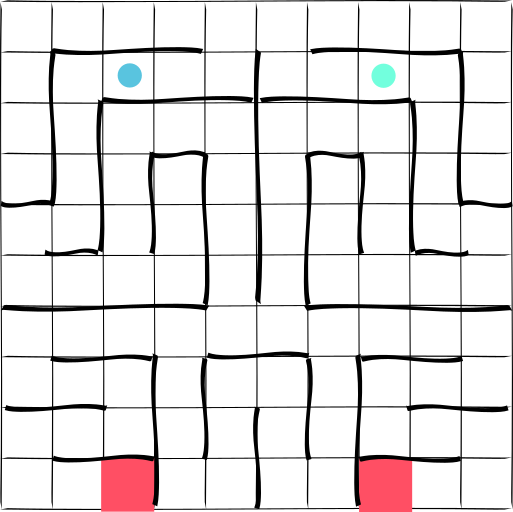
\includegraphics[width=0.5\textwidth,height=0.5\textheight]{../../pictures/drawings/maze.png}
\caption{maze.png}
\end{figure}

This reduces the state-action space by half!
\(\frac{1}{2}\mid S \mid \times \mid A \mid\). Note: just using state
abstraction it is not possible to achieve this reduction. Mirrored
states are not equivalent as the actions are inverted.

While other learners can still solve this problem. They miss out on
efficiency gains by abstracting first.

\hypertarget{related-work}{%
\subsubsection{Related work}\label{related-work}}

Other approaches to abstraction for RL focus on \ldots{}?

Near Optimal Behavior via Approximate State Abstraction \cite{Abel2017}
A Geometric Perspective on Optimal Representations for Reinforcement Learning \cite{Bellemare2019b}
successor representation

\hypertarget{discussion}{%
\subsection{Discussion}\label{discussion}}

But can we guarantee that these abstractions do not make it harder to
find the optimal policy? Is that even possible?

\begin{center}\rule{0.5\linewidth}{\linethickness}\end{center}

Want a general way (a function) to take an abstraction of an MDP
(defined by certain propreties) and return the difference between its
optimal policy and the true optimal policy. Want automated computational
complexity to solve this! Actually, we are not considering computational
complexity here only approximation error. For that can we just use
automatic differentiation!? Want a way to get bounds for all of these
combinations!

\begin{center}\rule{0.5\linewidth}{\linethickness}\end{center}

How do we know one policy is better than another? How do we know a
policy is optimal?

\[
\forall \pi\;\; V^{\pi^* } \ge V^{\pi} \\
\]

But, this definition of optimality implicitly assumes a uniform
distribution over states. This is unlikely. Rather, the distribution is
determined by the policy.

\[
\mathop{{\mathbb E}}_{s\sim D_{\pi}} \big[ V^{\pi^* } \big] \ge \mathop{{\mathbb E}}_{s\sim D_{\pi}} \big[ V^{\pi} \big] \\
D_{\pi}(s) = P(s | \pi) = \sum_{\text{all } \tau \text{ with } s_t = s} P(\tau | \pi)
\]

Now. How different is this?

I can imagine some degenerate solutions now being possible? Because we
can control the distribution we are being evaluated on. We could pick a
policy that oscillates between two states, never leaving the cycle.
Therefore it would have \(p(s_1) = p(s_2) = 0.5\) and
\(p(s_{i \neq 1,2}) = 0\).

That doesn't seem so bad?

\chapter{Symmetry}

% As recently noted by \cite{Caselles-Dupre2019}, ...

\chapter{Final remarks}\label{C:con}

\section{Summary}

While there do exist some tools for analysing abstractions for RL, we need better ones.
There are many unanswered questions (below), but, most importantly,
there is no well defined way to evaluate abstractions in general. {\color{red} doesnt quite work}

Linear Markov Decision Problems attempt to preserve the space of transition dynamics and the rewards.
But, they failed to preserve the value of the optimal actions, and thus cannot
guarantee performance in general. Ultimately, this was because the Bellman equation is non-linear.

We develop a measure of symmetry, and use it to give reinforcement learners a preference towards symmetry, a prior.
Our results did not show any advantage by using this prior, but due to computational and temporal\footnotemark constraints,
we were unable to make any conclusions.
% Symmetry attempts to preserve, ...?

\footnotetext{Temporal constraints meaning: A masters is a finite amunt of time.}

\newpage
\section{Future work}

There is a large amount of future work to be done if we want to:

\begin{displayquote}
\textit{understand how abstractions can increase the efficiency of reinforcement learning.}
\end{displayquote}

Our exploration of \textbf{Abstractions} in \ref{abstraction-rl}, raises a few fundamental questions;

\begin{itemize}
	\tightlist
	\item What is the advantage, if any, of \textit{state and action abstraction} versus \textit{state-action abstraction} \ref{exploit-abstraction-rl}?
	\item Of the two approaches to temporal abstraction, \textit{goal-like} and \textit{option-like} temporal abstraction, is one strictly better that the other? If not, then in which cases does \textit{goal-like} temporal abstraction perform better?
	\item Are the facets of evaluation presented in \ref{eval-abstractions} necessary and / or sufficient for 'efficient' performance of an abstraction in practice?
	\item Do many, or even all, abstractions of interest to RL live in the family defined in \ref{similar-classes}?
	\item Is there a difference between trajectory based similarity measures (that set the similarity $\chi(x, x')$ to be built from distances between the cumulants $D(c(x, \pi), c(x', \pi))$, rather than expected discounted cumulants $D(\mathcal C(x, \pi), \mathcal C(x, \pi))$)?
	\item What is the trade off (between computation and approximation error) of approximating $\int_{\pi \in \Pi}f(\pi)$ with $B \subset \Pi, \; \int_{\pi \in B}f(\pi)$?
	% How large does $X$ need to be to get a reliable estimate? Can we pick $X$ in intelligent, or random ways.
	\item What is necessary (rather than sufficient - which is proved in existing work) for the preservation of Bellman equation's ability to guide search? Can we weaken the requirements to: preserving the ordering of the value of optimal actions (rather than their absolute values as in existing work)?
\end{itemize}

Similarly, our results on \textbf{LMDPs} \ref{lmdp-validation} leave a few questions unanswered;

\begin{itemize}
	\tightlist
	\item In which cases does the LDMP give the right solution?
	\item What are the properties that make a MDP easily solvable (via LDMPs)?
	\item Can easily solvable MDPs (via LDMPs) be easily identified?
\end{itemize}

Finally, our results on \textbf{symmetric abstractions} \ref{symmetric-abstractions} leave a few questions unanswered;

\begin{itemize}
	\tightlist
	\item What is the (computational) efficiency of rejection sampling for symmetry biased distributions, and how does it scale with dimension? And how much data (sample efficiency) does that computation buy?
	% \item Rather than rejection sampling, use Metropolis-hastings. To allow to scale to higher dimensions.
	\item What happens if we use our measure of symmetry \ref{measure-symmetry} as a regulariser (as it is differentiable)?
	\item Invariants ...
	\item How can representations of states (or state-actions or ...) be ordered or structured? And how does this structure reduce the combinatorial space of possible symmetries?
	\item What is the cost of discovering temporal symmetries? How does this cost scale with the length of time? Can we amortize this cost by building symmetries from smaller symmetries in shorter sequences?
	% \item Run more rigorous experiments...
\end{itemize}

% % % % % % % % % % % % % % %
% Q: Number of integer factors as a function of n???
% Q: Efficiency of rejection sampling.
% Q: Relation to Lyapanov dynamics. Sampling distributions with gradient descent!??!
% Q: Proximity to symmetric states. How does this change as d increases?
% Q: Is there an advantage to building your temporal abstraction from k=n first, then to k=n+1.
% Q: Metro hastings. == RL?!? Pick transitions to help estimate a distribution?
% Q: With increasing k, does the topology of temporal abstractions always get coarser?



%%%%%%%%%%%%%%%%%%%%%%%%%%%%%%%%%%%%%%%%%%%%%%%%%%%%%%%

% and of course book style knows about backmatter
% \backmatter caused problems with appendices :-(
% and of course report style doesn't
%%%%%%%%%%%%%%%%%%%%%%%%%%%%%%%%%%%%%%%%%%%%%%%%%%%%%%%


%\bibliographystyle{ieeetr}
\bibliographystyle{acm}
\bibliography{mendeley}

\appendix
\chapter{Related work}

How do the topics considered in this thesis relate to the work done in the wider scientific community? Which work uses similar tools, which works build on the same foundations, which works have the same goals?

\hypertarget{related-work}{%
\section{Related work}\label{related-work}}

\hypertarget{mdps}{%
\paragraph{MDPs}\label{mdps}}

Dynamic programming, linear programming, \ldots{}?

\[
Q^{\pi}(s_0, a_0) = r(s_0, a_0)
+ \gamma \mathop{\text{max}}_{a_1} \mathop{\mathbb E}_{s_1\sim p(\cdot | s_0, a_0)} \Bigg[ r(s_1, a_1)
+ \gamma \mathop{\text{max}}_{a_2} \mathop{\mathbb E}_{s_2\sim p(\cdot | s_1, a_1)} \bigg[r(s_2, a_2)
+ \gamma \mathop{\text{max}}_{a_3} \mathop{\mathbb E}_{s_3\sim p(\cdot | s_2, a_2)} \Big[
\dots \Big] \bigg] \Bigg]
\]

\hypertarget{hrl}{%
\subparagraph{HRL}\label{hrl}}

Temoral abstractions of actions.(how does this related to a
decomposition of rewards) Ok, so we wany a multiscale representation?
Understanding how actions combine (this is necessary knowledge for HRL?)

Reasons to do HRL??? (want to verify these claims - and have refs for
them)

\begin{itemize}
\item
  credit assignment over long time periods (learning faster in one env)
\item
  exploration
\item
  transfer
\item
  To learn action abstractions they must capture info about the model.
  How much harder is it to learn action abstractions in model-free vs
  model-based settings?
\item
  Reward as a function of a subspace of the state space. (this is
  important for learning abstract representations and actions!?)
\item
  What do cts linear heirarchical actions look like!? and their loss
  surface!?
\item
  HLMDPs \cite{Saxea}
\item
  Modulated policy heirarchies \cite{Pashevich}
\item
  Model free representations for HRL \cite{Rafati}
\item
  \href{https://blog.aqnichol.com/2019/04/03/prierarchy-implicit-hierarchies/}{Prierarchy:
  Implicit Hierarchies}
\item
  Options
\item
  Near optimal representation learning for heirarchical RL \cite{Nachum2018}
\end{itemize}

Relation to pretraining / conditioning?

\begin{center}\rule{0.5\linewidth}{\linethickness}\end{center}

Why does Heirarchy (sometimes) work so well in reinforcement learning?

The authors claim that the benefits of HRL can be explained by better
exploration. However, I would interpret their results as saying; ``for
2D environments with walls, larger steps / actions result in greater
explration''. But what if the walls were replaced by cliffs? I imagine
this algorithm would do a lot worse!?

They also seem to misunderstand the main problem with HRL, discovery.
Once you have discovered a nice set of abstracted actions / a
representation, then yeah, you get faster reward propagation, better
exploration, \ldots{} etc.

\hypertarget{dynamic-programming}{%
\paragraph{Dynamic programming}\label{dynamic-programming}}

What is it? Memoized search. Why should we care?

\hypertarget{model-based-rl}{%
\subsection{Model-based RL}\label{model-based-rl}}

Pros and cons.

Model-based learning can be bad\ldots{} There may be many irrelevant
details in the environment that do not need to be modelled. A model-free
learning naturally ignores these things.

The importance of having an accurate model!

For example, let \(S\in R^n\) and \(A\in [0, 1]^n\). Take a transition
function that describes how a state-action pair generates a distribution
over next states \(\tau: S \times A \to \mathcal D(S)\). The reward
might be invariant to many of the dimensions.
\(r: X \times A -> \mathbb R\), where \(X \subset S\).

Thus, a model mased learner can have arbitrarily more to learn, by
attempting to learn the transition function. But a model-free learner
only focuses on \ldots{}

This leads us to ask, how can we build a representation for model-based
learning that matches the invariances in the reward function. (does it
follow that the invariances in reward fn are the invariances in the
value fn. i dont think so!?)

Take \(S \in R^d\) and let \(\hat S = S \times N, N \in R^k\). Where
\(N\) the is sampled noise. How much harder is it to learn
\(f: S \to S\) versus \(\hat f: \hat S \to \hat S\)?

https://arxiv.org/pdf/1903.00374v3.pdf https://arxiv.org/abs/1907.02057

\hypertarget{representation-learning-and-abstraction}{%
\subsection{Representation learning and
abstraction}\label{representation-learning-and-abstraction}}

The goal is to find a representation that decomposes knowledge into its
parts.

Another way to frame this is: trying to find the basis with the right
properties.

\begin{itemize}
\tightlist
\item
  sparsity,
\item
  independence,
\item
  multi scale,
\item
  locality/connectedness
\item
  ???
\end{itemize}


Types of abstraction for RL. Abstraction for efficient;

\begin{itemize}
\tightlist
\item
  exploration, [Learning latent state representation for speeding up exploration](https://arxiv.org/abs/1905.12621)
\item
  optimal control,
\item
  ???,
\end{itemize}


\subsection{Heirarchical reinforcement learning}


\end{document}
